\section{Introduction}
%-movivation
%-proposed

%\subsection{Motivation}
Visible light communications (VLC) have gained wide attention in the research community recently.
The possibilities of using every light emitting diode (LED) that already exists in our daily life to talk and to serve as
a new pervasive communication infrastructure are endless - it enables interference-free, secure, low cost, and energy efficient short range communications to a wide range of electronic devices and appliances, from cars with LED taillights, light fixtures with LED light bulbs, to refrigerators with tiny LED indicators. \autoref{fig:vlc-intro} illustrates how VLC works. VLC uses the optical signal to carry digital information by controlling the LED's light intensity in free space. When the light is transmitting, due to persistence of vision, human eyes cannot perceive the transmissions.

\begin{figure}[!t]
	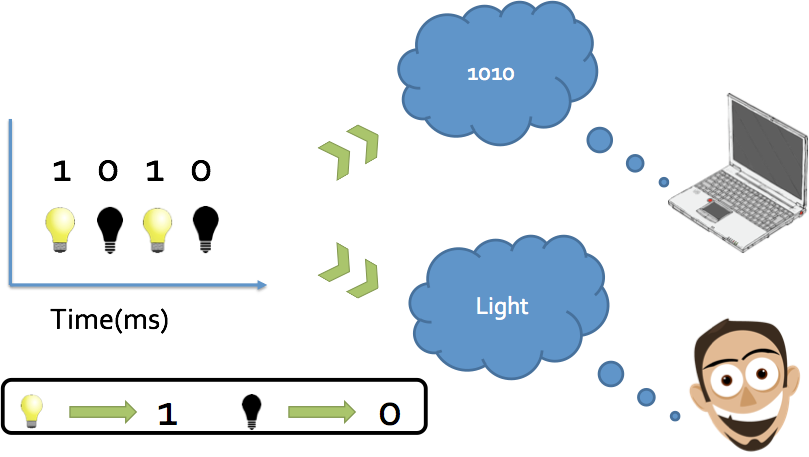
\includegraphics[scale=0.25]{fig/vlc_intro.png}
	\centering
	\caption{A schematic diagram of VLC}
	\label{fig:vlc-intro}
\end{figure}

This work implements a form of VLC that uses a \textbf{single LED} as the transmitter and a Complementary Mental-Oxide-Semiconductor (CMOS) \textbf{rolling shutter camera sensor} as the receiver, a form of Camera Communications (CamCom).
We chose to develop this form of VLC due to the universal availability of both the transmitting component - a simple LED (as opposed to an array of LEDs or an LCD screen), and the receiving component - a CMOS camera. 
Almost every modern mobile device, including smartphones, tablets, and laptops, is equipped with at least one built-in CMOS camera. 
We believe that this would be the best paradigm to jump-start the VLC technology in the market. 
As a result, one of the most important objectives of our work is to ensure the compatibility of a wide range of unmodified CMOS cameras to the LEDs transmission. 

% \begin{figure}[!htb]
% 	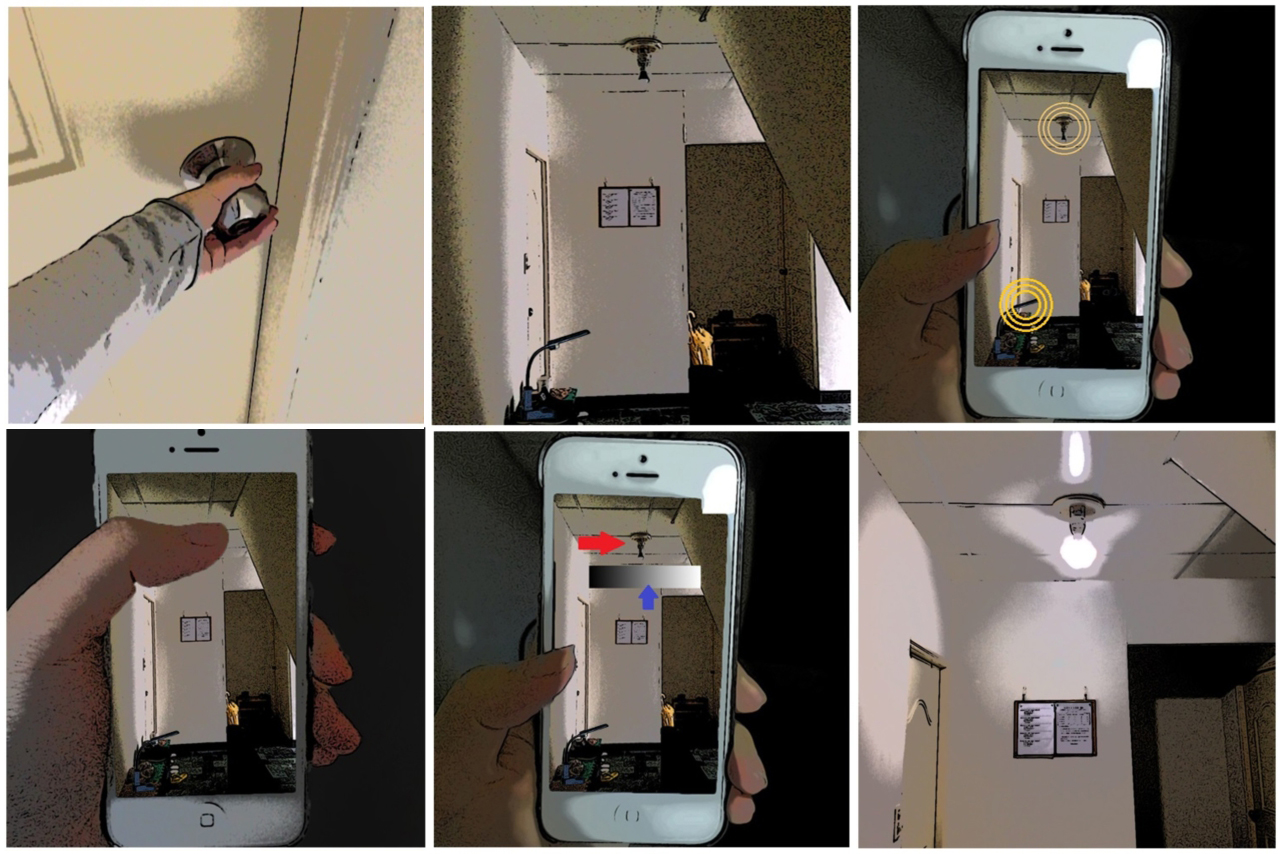
\includegraphics[scale=0.15]{fig/virtual_switch_hor.png}
% 	\centering
% 	\caption{An example of utilizing CamCom for visual association.}
% 	\label{fig:virtual_switch}
% \end{figure}


% Figure~\ref{fig:virtual_switch} shows a simple example. A user points her smartphone camera at multiple lights, touches the screen to select one, and uses the virtual switch that appears on the screen to adjust its lighting level. 
% In this scenario, the lights simply periodically transmit simple identifiers, such as IP addresses, to the smartphone. 
% The system is able to directly associate what the user sees (the image pixels mapped to the light selected by
% the user) to the transmission (the identifier of the light), and uses WiFi to sends the actual command to the right light to adjust the setting. 
% Compared to the conventional approach of identifying a particular set of visual features unique to the object with computer vision techniques, this approach is both simpler and more accurate.

% \begin{figure}[!htb]
% 	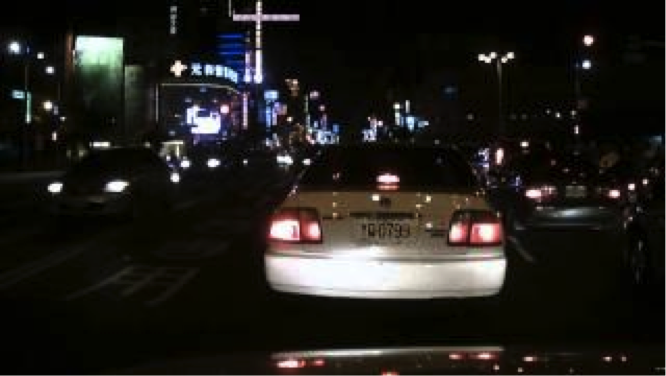
\includegraphics[scale=0.7]{fig/v2v.png}
% 	\centering
% 	\caption{An example of utilizing VLC for Vehicle communication.}
% 	\label{fig:v2v}
% \end{figure}

One very important advantage of CamCom is that the acquired images during the receiving process provide a means to \textbf{visually associate} the transmitting object with the transmissions, since the receiver has the knowledge of which pixels in the images are transmitting. We can use the idea in many applications. One is \textbf{Advanced Driver Assistance System (ADAS)}. we can use the LED tail lights of the front car to transmit a message to the camera of the rear cars. The message can contain safety-related status information, such as speed, location, heading, and brake/turn signal status, or user-specified short text messages to form an advanced driver assistance system. 

Another example is \textbf{indoor positioning}. We receive the light ID transmitted by the LED light and obtain the vertical distance between the receiver and the transmitting lights, and the horizontal distances between the lights. Then, we can calculate the relative position and know where we are in the building. 

We also can use the LED lights for \textbf{advertising}. For example, in a supermarket, we can use the LED light on the shelf to transmit the sale and discount information of the goods. We can use the traffic lights and signs to tell us the road status ahead. 

Besides, we can apply this kind of communication for \textbf{system diagnosis}. For example, when a scooter breaks down, we can transmit the sensor log via the LED tail lights to briefly check and detect the problem of the scooter; in a server room, full of machines on the racks, it is often hard to find out which server is having trouble, the nature of the problem, and the IP address of the machine. Imagine if each server has VLC capability on one of its high brightness LED, then we can point our smartphone's camera at an array of servers, and immediately these information will be shown right next to the server, for the administrator to diagnose the problem in an easier way.  

%\subsection{Main Components}
In this work, we presented a \textbf{theoretical model} to describe the single-LED-to-rolling-shutter-camera channel. Furthermore, we proposed the \textbf{Rolling Shutter-Frequency Shift Keying (RS-FSK) modulation} and demonstrated that the modulation is compatible to a wide range of CMOS cameras with different resolution, read-out time, and exposure time, satisfies the lighting requirements, and can be implemented with cost-efficient hardware.

However, as the transmitting light and the receiving camera are not synchronized, the transmitting frame rate and the receiving frame rate are not usually the same.
When the transmitting frame rate is higher than the receiving frame rate, there could be symbol loss.
When the transmitting frame rate is lower than the receiving frame rate, reception of redundant symbols is possible. 
Although no information is lost, the receiver still needs to detect the redundant symbol so that it can be dropped to obtained the correct symbol sequence.

A more common event when the transmitting frame duration and the receiving frame duration are different is that there could be multiple image areas each corresponding to a symbol. In other word, a mix of different symbols in a single received image frame. 
A mixed frame is a very common and periodic event.
Even when the transmitting and the receiving frame durations are very close to each other, mixed frames would be received because of the phase difference between transmitter and receiver.

Therefore, in this paper we present a scheme that can handle \textbf{unsynchronized} transmitter and receiver pairs. 
We also implement the entire system and evaluate whether packet reception rate can be improved.

